\section{Introduction}\label{sec:intro}

The four-vertex theorem says that the curvature of a simple closed plane curve
that is not a circle has two local maxima separated by two local minima,
with the values at both minima strictly smaller than those at both maxima.
Gluck~\cite[pp.~295--296]{Gluck1971} proved the converse for continuous
strictly positive curvature. Dahlberg~\cite[Theorem~1.1]{Dahlberg2005}
proved it for smooth signed curvature, provided the two selected maxima
are positive; see \cite{DGPV2007} for the history.

The four-vertex theorem has many discrete versions
\cite{Musin2004,OvsienkoTabachnikov2001,Sedykh1997,Tabachnikov2000,Dahlberg2008,Pak2010}.
In the one studied here the curvature at a vertex of a polygon is the
reciprocal radius of the circle through that vertex and its two neighbours.
Let $P$ be a convex $n$-gon, $n\ge 4$, with vertices $x_1,\dots,x_n$ in cyclic
order. Following Tabachnikov, call $P$ \emph{coherent} if for every $i$ the
center of the circle through $x_{i-1},x_i,x_{i+1}$ lies inside the angle of
$P$ at $x_i$. If $P$ is coherent and no four consecutive vertices lie on a
circle, then the cyclic sequence $r_1,\dots,r_n$ of the radii of these circles
has at least two local maxima and two local minima. This is due to
Musin (see \cite{Tabachnikov2000,Musin2004}); Dahlberg~\cite{Dahlberg2008}
proved a version for simple, locally regular polygons, not necessarily convex,
extending Bilinski's result for convex polygons with obtuse angles~\cite{Bilinski1963}.

In~\cite[Problem~2]{Tabachnikov2008} Tabachnikov posed the converse: a cyclic
sequence $r_1,\dots,r_n$ with at least two local maxima and two local minima
should be the radius sequence of a coherent convex polygon. Pak remarks
that he is not aware of a nontrivial discrete version of the converse
four-vertex theorem \cite[\S21.10, p.~206]{Pak2010}. We prove Tabachnikov's conjecture.

Local extrema are counted as by Dahlberg \cite{Dahlberg2008}. A
\emph{plateau maximum} of a cyclic sequence is a maximal run of equal
consecutive terms, not the whole sequence, whose two outside neighbours are
both strictly smaller. Plateau minima are defined in the same way. Two
extrema are \emph{distinct} if their runs are disjoint.

\begin{theorem}\label{thm:main}
Let $n\ge 4$ and let $r_1,\dots,r_n>0$ be a cyclic sequence with at least two
distinct plateau maxima and two distinct plateau minima. Then there is a
simple, strictly convex, coherent polygon $x_1,\dots,x_n$, listed
counterclockwise, whose circle through $x_{i-1},x_i,x_{i+1}$ has radius $r_i$
for every $i$.
\end{theorem}
% Lean: Gluck.Discrete.tabachnikov_converse_geometric (TabachnikovConverse.lean)

Strict convexity means that, for each edge, all other vertices lie in the
same open half-plane bounded by its supporting line; coherence places each
circumcenter in the interior of the corresponding vertex angle. The same
polygon has signed Menger curvature $1/r_i$.
Moreover, whenever $r_i\ne r_{i+1}$, the four vertices
$x_{i-1},x_i,x_{i+1},x_{i+2}$ do not lie on a common circle, independently of
whether other adjacent radii are equal.
% Lean: Gluck.Discrete.IsCoherentConvexPolygon.signedMengerR2_eq_inv_of_radii,
%       Gluck.Discrete.IsCoherentConvexPolygon.not_concyclic4_of_radius_ne
%       (TabachnikovCharacterization.lean)

Two distinct plateau maxima already force two distinct plateau minima, and
conversely (Lemma~\ref{lem:dfv-plateau}), so either half of the hypothesis
suffices.

\begin{figure}[t]
\centering
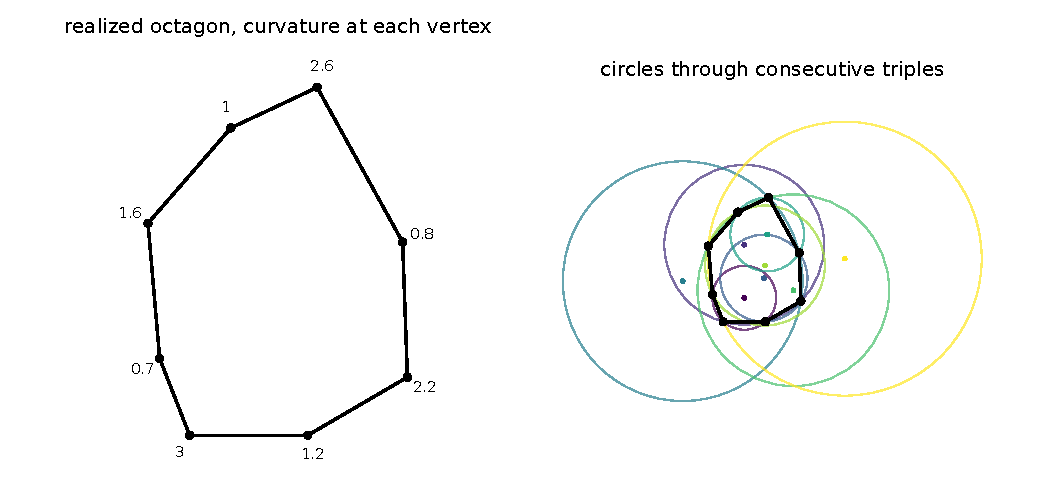
\includegraphics[width=0.7\textwidth]{tabachnikov/figures/example.pdf}
\caption{A coherent convex octagon realizing the curvatures
$(3,1.2,2.2,0.8,2.6,1,1.6,0.7)$, and its eight circles through consecutive
vertex triples, whose centers lie inside the vertex angles. Computed
numerically and checked to double precision.}
\label{fig:example}
\end{figure}

Figure~\ref{fig:example} shows an example. The theorem is sharp:

\begin{corollary}\label{cor:iff}
Let $n\ge4$, and let $r_1,\dots,r_n$ be positive numbers that are not all
equal. Then $r$ is the radius sequence of a coherent convex polygon if and
only if $r$ has two distinct
plateau maxima and two distinct plateau minima.
\end{corollary}

\begin{proof}
One direction is Theorem~\ref{thm:main}. Conversely, a coherent convex
polygon is simple, and its circumcenters lie in the closed vertex sectors,
which is Dahlberg's local regularity \cite{Dahlberg2008}. It is
not inscribed in a circle, since otherwise all the circles through
consecutive triples would coincide and $r$ would be constant. Dahlberg's
discrete four-vertex theorem \cite{Dahlberg2008}, whose extrema
are plateau extrema with distinct runs, gives the two maxima and two minima.
Only its convex case is needed here, since the polygon is strictly convex.
The formalization includes this forward implication and the equivalence.
% Lean: Gluck.Discrete.tabachnikov_radius_characterization
\end{proof}

\begin{remark}[The wording of the problem]\label{rem:wording}
Read with strict extrema, $r_{i-1}<r_i>r_{i+1}$, Tabachnikov's hypothesis
is a special case of Theorem~\ref{thm:main}. Read with weak extrema,
$r_{i-1}\le r_i\ge r_{i+1}$, the statement is false: $r=(2,1,1,1)$ has the
weak local maxima $r_1,r_3$ and minima $r_2,r_4$ but one plateau maximum, so
by Corollary~\ref{cor:iff} it is not a radius sequence. Constant
sequences are excluded by our plateau convention and are realized by regular
$n$-gons.
Tabachnikov's non-concyclicity hypothesis holds for our polygon exactly when
$r_i\ne r_{i+1}$ for all $i$: one implication was just noted, and if
$r_i=r_{i+1}$ in a coherent convex polygon, the circles at $x_i$ and $x_{i+1}$ share the chord
$x_ix_{i+1}$, the radius and the side of their centers, so they coincide.
\end{remark}

It is convenient to work with the curvatures $\kappa_i=1/r_i$. The hypothesis
of Theorem~\ref{thm:main} is then equivalent to a \emph{strict four-vertex
window}: indices $i_1<i_2<i_3<i_4<i_1+n$ and a level $c$ with
\begin{equation}\label{eq:dfv}
  \kappa_{i_2},\ \kappa_{i_4} \;<\; c \;<\; \kappa_{i_1},\ \kappa_{i_3}.
\end{equation}

\subsection*{Organization}
Section~\ref{sec:method} explains the construction informally; the proof
occupies Sections~\ref{sec:setup}--\ref{sec:constructions} and
Appendix~\ref{sec:elimination}. Section~\ref{sec:continuity} shows that the
polygon can be chosen to depend in a $C^1$ way on the data near every
nonconstant admissible sequence (Theorem~\ref{thm:local}), but that a global
continuous choice does not exist, even along a path of admissible
nonconstant hexagon data (Theorem~\ref{thm:hexagon}); the obstruction is the
radius of the smallest enclosing circle. Theorems~\ref{thm:main},
\ref{thm:local} and~\ref{thm:hexagon} are formalized in Lean~4 with Mathlib
\cite{GluckLean}; Appendix~\ref{sec:lean} lists the formal statements.

Tabachnikov also conjectured a converse for the radii of the circles tangent
to three consecutive sides, the discrete four-vertex theorem of
Wegner~\cite{Wegner1994,Tabachnikov2000}; the companion conjecture is also
stated in \cite[Problem~2]{Tabachnikov2008}. Section~\ref{sec:side-tangent} proves this companion converse for inward
circles tangent to the three supporting lines, including their extensions.
It does not use the four-length system of the main theorem.
Section~\ref{sec:discussion} gives a counterexample to the four-vertex theorem
for turning-angle curvature. It also gives a counterexample to the naive
converse for signed Menger curvature and asks what additional hypotheses
are needed for that converse.
